\uuid{xlOX}
\exo7id{7114}
\titre{exo7 7114}
\auteur{megy}
\organisation{exo7}
\datecreate{2017-01-21}
\isIndication{true}
\isCorrection{true}
\chapitre{Géométrie affine euclidienne}
\sousChapitre{Géométrie affine euclidienne du plan}
\module{Géométrie}
\niveau{L2}
\difficulte{}

\contenu{
\texte{
% tags : similitude
Soit $ABC$ un triangle isocèle en $A$, $A'$ et $B'$ les pieds des hauteurs issues de $A$ et $B$, $I$ le milieu de $[CB']$ et $J$ le milieu de $[A'I]$. Montrer que $(BI)$ et $(AJ)$ sont orthogonales.

\begin{center}
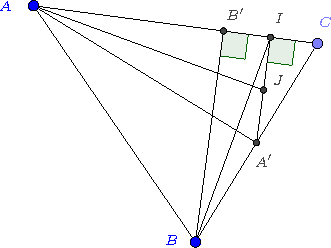
\includegraphics{../images/pdf/xlOX-1.pdf}
\end{center}
}
\indication{Utiliser une similitude.}
\reponse{
Les triangles $AA'I$ et $BB'C$ sont semblables, par une similitude d'angle $\pi/2$. L'image de $(AJ)$ par cette similitude est $(BI)$.
}
}
